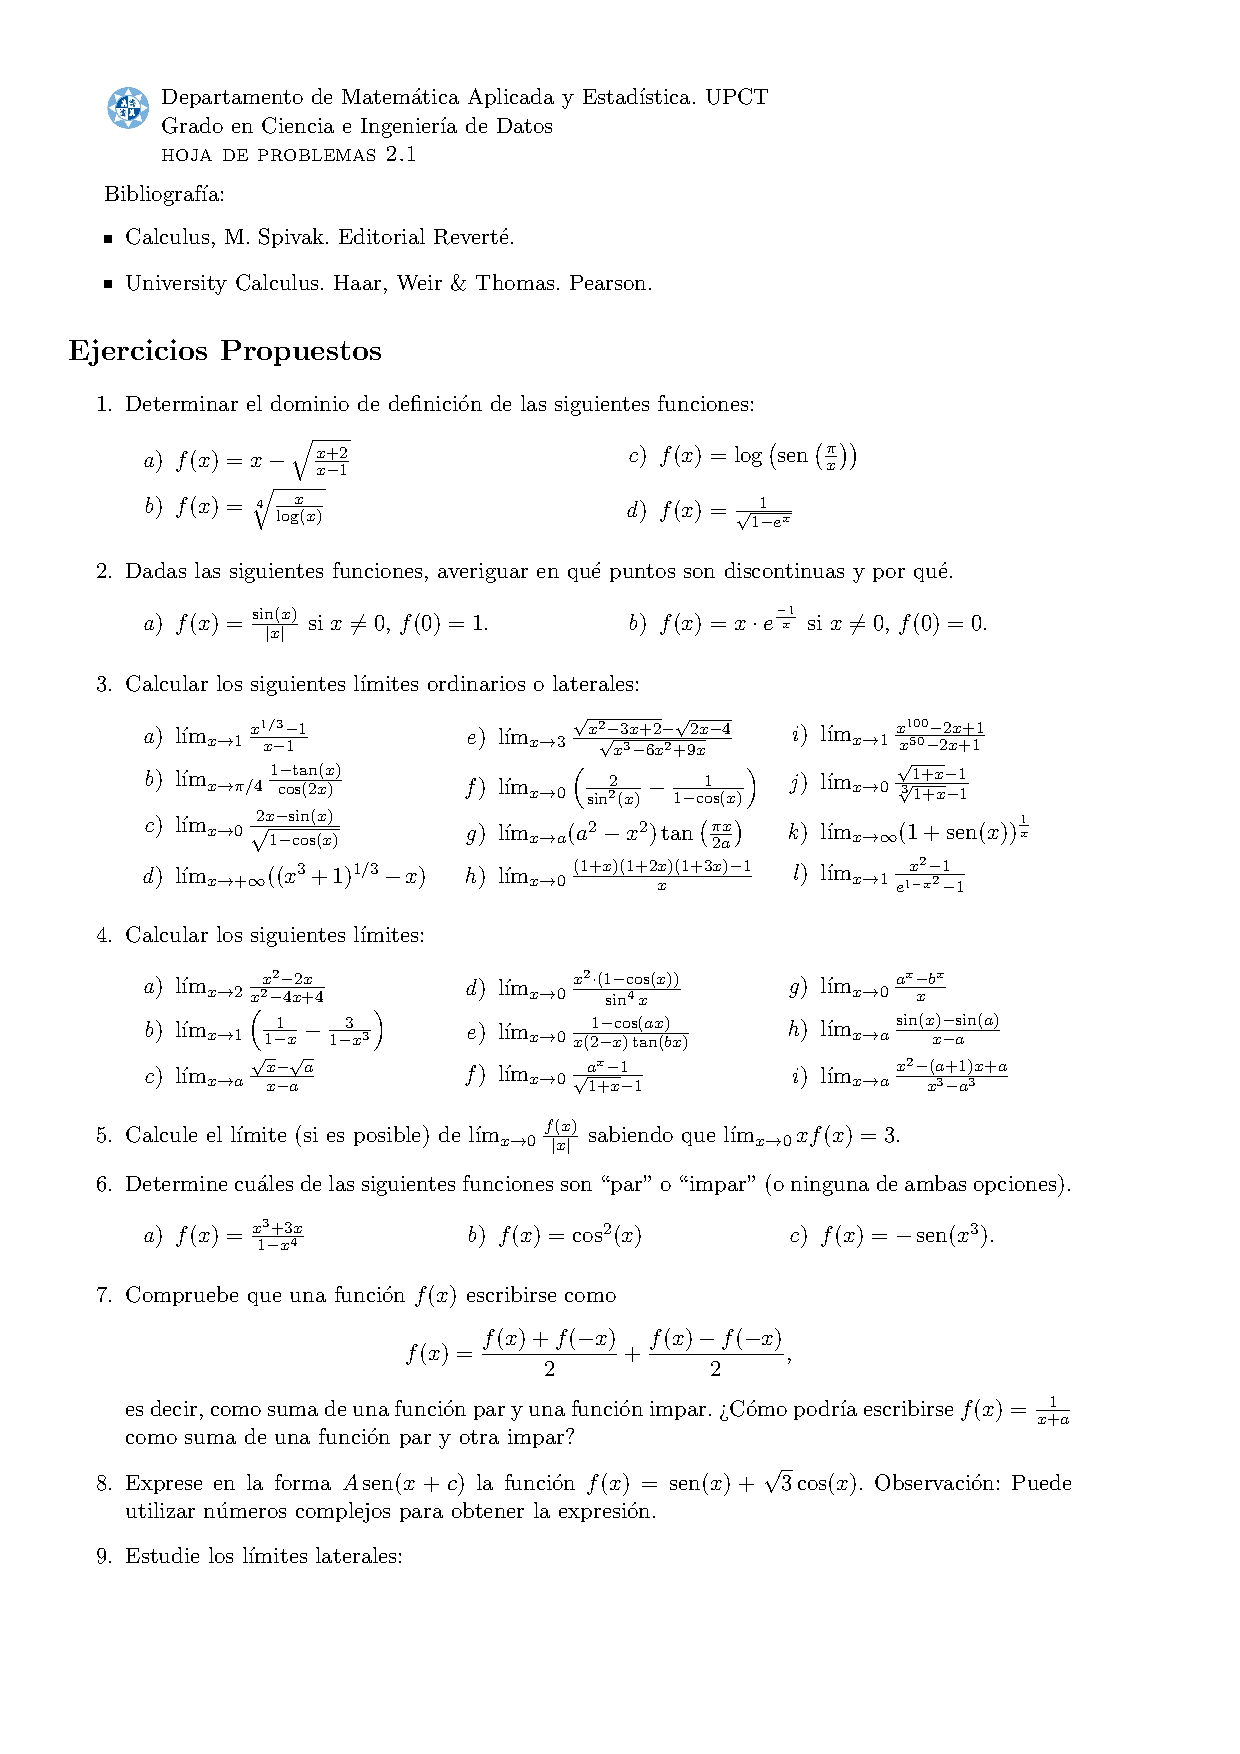
\includepdf[pages=-]{"Tema 2/Hoja 2.1/Hoja 2.1.pdf"}

\begin{enumerate}[label=\color{red}\textbf{\arabic*)}, leftmargin=*]
	\item \textcolor{lightblue}{Determinar el dominio de definición de las siguientes funciones:}
	\begin{enumerate}[label=\color{red}\alph*)]
		\item \textcolor{blue}{$f(x)=x-\sqrt{\dfrac{x+2}{x-1}}$}
		
		$\dfrac{x+2}{x-1}\ge 0$\qquad \begin{tikzpicture}[baseline=(current bounding box.center)]
			\draw (-3, 0) -- (2,0);
			\foreach \x in {-2,1} {
			\fill[lightblue] (\x, 0) circle (2pt)  node[above] {$\x$};
			};
			\node[below] at (-2.5,0) {Sí};
			\node[below] at (1.5,0) {Sí};
			\node[below] at (-0.5,0) {No};
			\node[above] at (-2.5,0.2) {$\frac{-}{-}=+$};
			\node[above] at (1.6,0.2) {$\frac{+}{+}=+$};
			\node[above] at (-0.5,0.2) {$\frac{+}{-}=-$};
		\end{tikzpicture}
		
		$\mathrm{Dom}(f)=(-\infty,-2]\cup(1,+\infty)$
		\item $\textcolor{blue}{f(x)=\sqrt[4]{\dfrac{x}{\log(x)}}}$
		
		$\begin{array}{l}
			\dfrac{x}{\log(x)}\ge0\\
			x>0\\
			\mathrm{Dom}(f)=(1,+\infty)
		\end{array}$\qquad\begin{tikzpicture}[baseline=(current bounding box.center)]
		\draw (-1,0) -- (2,0);
		\foreach \x in {0,1}{
		\fill[lightblue] (\x,0) circle (2pt) node[above] {$\x$};
		}
		\node[below] at (0.5,0) {No};
		\node[below] at (1.5,0) {Si};
		\end{tikzpicture}
		
		\begin{tikzpicture}% function
			\begin{axis}[xlabel=x,ylabel=y, axis lines=center]
				\addplot[lightblue, samples=150] {x/ln(x)};
			\end{axis}
		\end{tikzpicture}
		
		\item $\textcolor{blue}{f(x)=\log\left(\sin\left(\dfrac{\pi}{x}\right)\right)}$
		
		\begin{tikzpicture}% function
			\begin{axis}[xlabel=x,ylabel=y, axis lines=center]
				\addplot[lightblue, samples=150] {ln(sin(pi/x))};
			\end{axis}
		\end{tikzpicture}
		
		\item $\textcolor{blue}{f(x)=\dfrac{1}{\sqrt{1-e^x}}}$
	\end{enumerate}
	\item \textcolor{lightblue}{Dadas las siguientes funciones, averiguar en qué puntos son discontinuas y por qué.}
	\begin{enumerate}[label=\color{red}\alph*)]
		\item \textcolor{blue}{$f(x)=\dfrac{\sin(x)}{|x|}$ si $x\neq0,\,f(0)01$}
		
		$f(x)=\begin{cases}
			\dfrac{\sin(x)}{|x|} & \text{si }x\neq0\\
			1 & \text{si }x=0
		\end{cases}$
		
		$\begin{array}{l}
			\lim_{x\to0^+}\dfrac{\sin(x)}{|x|}=\lim_{x\to0^+}\dfrac{\sin(x)}{x}=\left\{\sin(x)\equiv x\quad(x\to0)\right\}=\lim_{x\to0^+}\dfrac{x}{x}=1\\
			\lim_{x\to0^-}\dfrac{\sin(x)}{|x|}=\lim_{x\to0^-}\dfrac{\sin(x)}{-x}=\lim_{x\to0}\dfrac{x}{-x}=-1
		\end{array}$
		
		No es continua en $x=0$ porque el límite no existe $\longrightarrow$ Discontinuidad de salto finito.
		
		(Hay continuidad lateral por la derecha)
		
		\item \textcolor{blue}{$f(x)=x\cdot e^{\frac{-1}{x}}$ si $x\neq0\,f(0)=0$.}
		
		$f(x)=\begin{cases}
			x\cdot e^{\frac{-1}{x}} & \text{si } x\neq0\\
			0 & \text{si }x=0
		\end{cases}$
		
		$ \begin{array}{l}
			\lim_{x\to0^+}x\cdot e^{\frac{-1}{x}}=0\\
			\begin{aligned}
				\lim_{x\to0^-}x\cdot e^{\frac{-1}{x}}&=\lim_{x\to0^-}\dfrac{e^{\frac{-1}{x}}}{\frac{1}{x}}=\lim_{x\to0^-}\dfrac{x}{e^{\frac{-1}{x}}}=\left\{\begin{array}{l}
				\frac{1}{x}=t\\
				\lim_{x\to0^-}t=-\infty
			\end{array}\right\}\\
			&=\lim_{t\to-\infty}\dfrac{e^{-t}}{t}=\{\text{L'Hôpital}\}=\lim_{t\to-\infty}\dfrac{-e^{-t}}{1}=\lim_{t\to-\infty}e^{-t}=\bboxed{0}
			\end{aligned}
		\end{array}$
	\end{enumerate}
	\item \textcolor{lightblue}{Calcular los siguientes límites ordinarios o laterales:}
	\begin{enumerate}[label=\color{red}\alph*)]
		\item $\textcolor{blue}{\lim_{x\to1}\dfrac{x^{\frac{1}{3}}-1}{x-1}=}$
		\item $\textcolor{blue}{\lim_{x\to\frac{\pi}{4}}\dfrac{1-\tan(x)}{\cos(2x)}=}\lim_{x\to\frac{\pi}{4}}\dfrac{1-\dfrac{\sin(x)}{\cos(x)}}{\cos^2(x)-\sin^2(x)}=\lim_{x\to\frac{\pi}{4}}\dfrac{\dfrac{\cos(x)-\sin(x)}{\cos(x)}}{(\cos(x)-\sin(x))\cdot(\cos(x)+\sin(x))}$
		
		$=\lim_{x\to\frac{\pi}{4}}\dfrac{1}{\cos(x)\cdot(\cos(x)+\sin(x)}=\dfrac{1}{\frac{\sqrt{2}}{2}\cdot\sqrt{2}}=1$
		\item $\textcolor{blue}{\lim_{x\to0}\dfrac{2x-\sin(x)}{\sqrt{1-\cos(x)}}=}\left\{1-\cos(x)\equiv\dfrac{x^2}{2}\quad(x\to0)\right\}=\dfrac{2x-\sin(x)}{\sqrt{\frac{x^2}{2}}}=\lim_{x\to0}\dfrac{2x-\sin(x)}{\frac{|x|}{\sqrt{2}}}=$
		
		$\begin{cases}
		\lim_{x\to0^+}\sqrt{2}\left(\dfrac{2x-\sin(x)}{x}\right)=\lim_{x\to0^+}\sqrt{2}\left(2-\dfrac{\sin(x)}{x}\right)=2\sqrt{2}\sqrt{2}\,\lim_{x\to0^+}\dfrac{\sin(x)}{x}=2\sqrt{2}-\sqrt{2}=\bboxed{\sqrt{2}}\\
		\lim_{x\to0^-}\sqrt{2}\left(\dfrac{2x-\sin(x)}{-x}\right)=-\sqrt{2}
		\end{cases}$
		\item $\textcolor{blue}{\lim_{x\to\infty}(x^3+1)^{\frac{1}{3}}-x=}\lim_{x\to+\infty}x\cdot\left( \left(\dfrac{(x^3+1)}{x^3}\right)^{\frac{1}{3}}-1\right)=\lim_{x\to+\infty}\left(\left(1+\dfrac{1}{x^3}\right)^{\frac{1}{3}}-1\right)$
		
		$=\left\{t=\dfrac{1}{x^3}\quad t\xrightarrow[x\to\infty]{}0\right\}=\lim_{x\to+\infty}x\cdot\dfrac{1}{3}\cdot\dfrac{1}{x^3}=\lim_{x\to+\infty}\dfrac{1}{3x^2}=\bboxed{0}$
		\item $\textcolor{blue}{\lim_{x\to3}\dfrac{\sqrt{x^2-3x+2}-\sqrt{2x-4}}{\sqrt{x^3-6x^2+9x}}=}\lim_{x\to3}\dfrac{\sqrt{x-1}\sqrt{x-2}-\sqrt{2}\sqrt{x-2}}{\sqrt{x}\sqrt{(x-3)^2}}=\lim_{x\to3}\dfrac{\sqrt{x-2}\cdot(\sqrt{x-1}-\sqrt{2})}{\sqrt{x}\cdot|x-3|}=\lim_{x\to3}\dfrac{\sqrt{x-1}-\sqrt{2}}{\sqrt{3}\cdot|x-3}=\begin{cases}
			\lim_{x\to3^+}\dfrac{\sqrt{x-1}-\sqrt{2}}{\sqrt{3}\cdot(x-3)}=\left\{\text{L'Hôpital}\right\}=\lim_{x\to3^+}\dfrac{\frac{1}{2\sqrt{x-1}}}{\sqrt{3}}=\dfrac{1}{2\sqrt{6}}\\
			\lim_{x\to3^-}\dfrac{\sqrt{x-1}-\sqrt{2}}{-\sqrt{3}\cdot(3-x)}=-\dfrac{1}{2\sqrt{6}}
		\end{cases}\longrightarrow\bboxed{\nexists\lim}$
		
		$\begin{aligned}
			x^2-3x+2&=(x-1)(x-2)\\
			2x-4&=2\cdot(x-2)\\
			x^3-6x^2+9x&=x\cdot(x-3)^2
		\end{aligned}$
		\item $\textcolor{blue}{\lim_{x\to0}\left(\dfrac{2}{\sin^2(x)}-\dfrac{1}{1-\cos(x)}\right)=}\lim_{x\to0}\dfrac{2(1-\cos(x))-\sin^2(x)}{\sin^2(x)\cdot(1-\cos(x))}=\left\{\begin{array}{c}
			\sin(x)\equiv x\quad(x\to0)\\
			1-\cos(x)\equiv\frac{x^2}{2}\quad(x\to0)
		\end{array}\right\}=\lim_{x\to0}\dfrac{2-2\cos(x)-\sin^2(x)}{x^2\cdot\frac{x^2}{2}}=\lim_{x\to0}\dfrac{2-2\cos(x)-1+\cos^2(x)}{\frac{x^4}{2}}=\lim_{x\to0}\dfrac{(\cos(x)-1)^2}{\frac{x^4}{2}}=\lim_{x\to0}\dfrac{\left(\frac{x^2}{2}\right)^2}{\frac{x^4}{2}}=\bboxed{\dfrac{1}{2}}$
		\item $\textcolor{blue}{\lim_{x\to a}(a^2-x^2)\tan\left(\dfrac{\pi x}{2a}\right)=}\lim_{x\to a}(a-x)(a+x)\cdot\dfrac{\sin\left(\frac{\pi x}{2a}\right)}{\cos\left(\frac{\pi x}{2a}\right)}=\lim_{x\to a}2a(x-a)\dfrac{1}{\cos\left(\frac{\pi x}{2a}\right)}=2a\cdot\lim_{x\to a}\dfrac{a-x}{\cos\left(\frac{\pi x}{2a}\right)}=\left\{\text{L'Hôpital}\right\}=2a\cdot\lim_{x\to0}\dfrac{-1}{-\sin\left(\frac{\pi x}{2a}\right)\cdot\frac{\pi}{2a}}=\bboxed{\dfrac{4a^2}{\pi}}$
		\item $\textcolor{blue}{\lim_{x\to0}\dfrac{(1+x)(1+2x)(1+3x)-1}{x}=}\lim\dfrac{x\cdot(x+2x+3x)}{x}=1+2+3=\bboxed{6}$
		
		$\dfrac{ax^3+bx^2+cx+d}{x}=\dfrac{ax^3+bx^2+cx+\cancel{1}-\cancel{1}}{x}=\dfrac{\cancel{x}\cdot(ax^2+bx+c)}{\cancel{x}}=ax^2+bx+c\quad (x\to0)$
		\item $\textcolor{blue}{\lim_{x\to1}\dfrac{x^{100}-2x+1}{x^{50}-3x-1}=}\lim_{x\to1}\dfrac{\cancel{(x-1)}\cdot(x^{99}+x^{98}+\cdots+x+1)}{\cancel{(x-1)}\cdot(x^{99}+x^{98})+\cdots+x+1}=\dfrac{98}{48}$
		
		$\begin{array}{c|ccccccc}
			& 100 & 99 & 98 & \cdots & 2 & 1 & 0 \\
			& 1 & 0 & 0 &  & 0 & -2 & 1 \\
			1 &  & 1 & 1 &  & 1 & 1 & -1 \\ \hline
			& 1 & 1 & 1 & \cdots & 1 & -1 & \multicolumn{1}{|c}{0}\\
		\end{array}$
		\item $\textcolor{blue}{\lim_{x\to\infty}\dfrac{\sqrt{1+x}-1}{\sqrt[3]{1+x}-1}=}\lim_{x\to0}\dfrac{\frac{1}{2}\cdot x}{\frac{1}{3}\cdot x}=\bboxed{\dfrac{3}{2}}$
		\item $\textcolor{blue}{\lim_{x\to\infty}\left(1+\sin(x)\right)^{\frac{1}{x}}=}\lim_{n\to\infty}{\Huge e}^{\frac{1}{x}\log(1+\sin(x))}=\left\{1+\sin(x)=\dfrac{\pi}{2}+2\pi\quad(x\to+\infty)\right\}=1$
		\item $\textcolor{blue}{\lim_{x\to1}\dfrac{x^2-1}{e^{1-x^2}-1}=}\lim_{x\to1}\dfrac{x^2-1}{e^{1-x^2}-1}=\lim_{x\to1}\dfrac{(x-1)(x+1)}{e^{(1-x)(1+x)}-1}=\lim_{x\to1}\dfrac{2\cdot(x-1)}{e^{2(x-1)}-1}=\lim_{x\to1}\dfrac{\cancel{2}}{-\cancel{2}e^{2(x-1)}}=\bboxed{-1}$
	\end{enumerate}
	\item \textcolor{lightblue}{Calcular los siguientes límite:}
	\begin{enumerate}[label=\color{red}\alph*)]
		\item $\textcolor{blue}{\lim_{x\to2}\dfrac{x^2-2x}{x^2-4x+4}=}$
		\item $\textcolor{blue}{\lim_{x\to1}\left(\dfrac{1}{x-1}-\dfrac{3}{1-x^3}\right)=}$
		\item $\textcolor{blue}{\lim_{x\to a}\dfrac{\sqrt{x}-\sqrt{a}}{x-a}=}\bboxed{\dfrac{1}{2\sqrt{a}}}$
		\item $\textcolor{blue}{\lim_{x\to0}\dfrac{x^2\cdot(1-\cos(x))}{\sin^4x}=}$
		\item $\textcolor{blue}{\lim_{x\to0}\dfrac{1-\cos(ax)}{x(2-x)\tan(bx)}=}$
		\item $\textcolor{blue}{\lim_{x\to0}\dfrac{a^x-1}{\sqrt{1+x}-1}=}$
		\item $\textcolor{blue}{\lim_{x\to0}\dfrac{a^x-b^x}{x}=}$
		\item $\textcolor{blue}{\lim_{x\to a}\dfrac{\sin(x)-\sin(a)}{x-a}=}$
		\item $\textcolor{blue}{\lim_{x\to a}\dfrac{x^2-(a+1)x+a}{x^3-a^3}=}$
	\end{enumerate}
	\item \lb{Calcule el límite (si es posible) de $\lim_{x\to}\dfrac{f(x)}{|x|}$ sabiendo que $\lim_{x\to0}xf(x)=3$}
	
	$\begin{array}{l}
		f(x)=\dfrac{3}{x}\\
		\lim_{x\to0}x\cdot f(x)=3\\
		\lim_{x\to0}\dfrac{3}{x\cdot|x|}=\begin{cases}
			\lim_{x\to0^+}\dfrac{3}{x^2}=+\infty\\
			\lim_{x\to0^-}\dfrac{3}{-x^2}=-\infty
		\end{cases}\longrightarrow\bboxed{\nexists\lim}
	\end{array}$
	\item \lb{Determine cuáles de las siguientes funciones son "par" o "impar" (o ninguna de ambas proposiciones).}
	\begin{enumerate}[label=\color{red}\alph*)]
		\item $\db{f(x)=\dfrac{x^3+3x}{1-x^4}}\quad$ Impar
		
		$f(-x)=\dfrac{(-x)^3+2\cdot(-x)}{1-(-x)^4}=\dfrac{-x^3-3x}{1-x^4}=\dfrac{-(x^3+3)}{1-x^4}=-f(x)$
		\item $\db{f(x)=\cos^2(x)=}$
		\item $\db{f(x)=-\sin(x^3)=}$
	\end{enumerate}
	\item \lb{Compruebe que una función $f(x)$ escribirse como \[ f(x)=\dfrac{f(x)-f(-x)}{2}+\dfrac{f(x)-f(-x)}{2}, \] es decir, como suma de una función par y otra impar. ¿Cómo podría escribirse $f(x)=\dfrac{1}{x-a}$ como suma de una función par y otra impar?}
	
	Efectivamene la igualdad se cumple y $g(x)=\dfrac{f(x)-f(-x)}{2}$ es par, ya que $g(-x)=g(x)$. Por otra parte $h(x)=\dfrac{f(x)-f(-x)}{2}$ es impar, puesto que $h(-x)=\dfrac{f(-x)-f(x)}{2}=-h(x)$
	
	Ahora, \[ \dfrac{1}{x+1} =\dfrac{1}{2}\cdot\left(\dfrac{1}{x+a}+\dfrac{1}{-x+a}\right)+\dfrac{1}{2}\cdot\left(\dfrac{1}{x+a}-\dfrac{1}{-x+a}\right)=\dfrac{a}{a^2+x^2}+\dfrac{-x}{a^2-x^2}.\] Ahora $g(x)=\dfrac{a}{a^2-x^2}$ es par y $(x)=\dfrac{-x}{a^2-x^2}$
	\item \lb{Exprese en la forma $A\sin(x+c)$ la función $f(x)=\sin(x)+\sqrt{3}\cos(x)$. Observación: Puede utilizar números complejos para obtener la expresión.}
	
	$\begin{array}{l}
		f(x)=\sin(x)+\sqrt{3}\cos(x)=A\sin(x+c)\\
		e^{ix}=\cos(x)+\imath\sin(x)\\
		\sin(x)=\dfrac{e^{ix}-e^{-ix}}{2\imath}\qquad\cos(x)=\dfrac{e^{ix}-e^{-ix}}{2}\\
		\begin{aligned}
			f(x)&=\dfrac{e^{ix}-e^{-ix}}{2\imath}+\sqrt{3}\cdot\dfrac{e^{ix}-e^{-ix}}{2}\\
			&=\dfrac{e^{ix}-e^{-ix}+\sqrt{3}\imath\cdot e^{ix}+\sqrt{\imath\cdot e^{-ix}}}{2\imath}=\dfrac{e^{ix}\overbrace{(1+\sqrt{3}\imath)}^{2\cdot e^{\frac{\pi}{3}}}-e^{-ix}\overbrace{(1-\sqrt{3}\imath)}^{2\cdot e^{-\frac{\pi}{3}\imath}}}{2\imath}\\
			&=2\cdot\left(\dfrac{e^{\imath\left(x+\frac{\pi}{3}\right)}-e^{-\imath\left(x+\frac{\pi}{3}\right)}}{2\imath}\right)
		\end{aligned}
	\end{array}$
	\item \lb{Estudie los límites laterales:}
	\begin{enumerate}[label=\color{red}\alph*)]
		\item \db{$f(x)=\dfrac{|x|}{x^2+x}$ en $x=0$.}
		\item \db{$f(x)=e^{\frac{|x|}{x}}$ en $x=0$.}
		\item \db{$f(x)=\dfrac{1+e^{\frac{1}{x}}}{1-e^{\frac{1}{x}}}$ en $x=0$.}
	\end{enumerate}
	\item \lb{Calcule los siguientes límites:}
	\begin{enumerate}[label=\color{red}\alph*)]
		\item $\db{\lim_{n\to\infty}\sqrt[n]{(x+a_1)(x+a_2)\dots(x+a_n)}-x=}$
		\item $\db{\lim_{n\to\infty}x(\sqrt[x]{2}-1)=}$
		\item $\db{\lim_{x\to0}(\cos(ax))^{\frac{1}{x^2}}=}$
	\end{enumerate}
	\item \lb{Estudie la continuidad de la función: \[ f(x)=\begin{cases}
			\dfrac{1}{x}\log\left(\dfrac{1+x}{1-x}\right) & \text{si }-1<x<1\\
			0 & \text{si }x=0
		\end{cases} \]}
	\item \lb{Halle los siguientes límites en función del número $\alpha=\lim_{x\to0}\dfrac{\sin(x)}{x}.$}
	\begin{enumerate}[label=\color{red}\alph*)]
		\item $\db{\lim_{n\to\infty}\dfrac{\sin(x)}{x}=}$
		\item $\db{\lim_{n\to\infty}x\sin\left(\dfrac{1}{x}\right)=}$
	\end{enumerate}
	\item \lb{Demuestre que existe algún número $x$ tal que \[ \sin(x)=x-1. \]}
	\item \lb{Determinar los valores del número real $k$ para los cuales la función $p(x)=x^3-3x+k$ se anula en algún punto del intervalo $[-1,1]$.}
	\item \lb{Estudiar la existencia y la continuidad de la función inversa de la función $f(x)=3+\dfrac{1}{x}$ definida para $x>0$.}
	\item \lb{Estudiar la existencia y la continuidad de la función inversa de la función $f(x)=\dfrac{1-x^3}{x^3}$ definida para $x>1$.}
\end{enumerate}